\documentclass[a4paper, 10pt]{article}
\usepackage[T1]{fontenc}
\usepackage[utf8]{inputenc}
\usepackage[slovene]{babel}
\usepackage{csquotes}
\usepackage{lmodern}
\usepackage{amsmath}
\usepackage{leftidx}
%\usepackage[backend=biber, style=numeric]{biblatex}
\usepackage{amssymb}
\usepackage{amsthm}
\usepackage{amsfonts}
\usepackage{graphicx}
\usepackage{wrapfig}
\usepackage{amsthm}
\usepackage{mathrsfs}
\usepackage{mathtools}
\usepackage{url}
\usepackage{subfigure}
\usepackage{multirow}
\usepackage{lipsum}
\usepackage{wrapfig}
\usepackage{tikz}
\usepackage[format=plain, font=small, labelfont=bf, textfont=it, justification=centerlast]{caption}
\usepackage{booktabs}
\usepackage{siunitx}
%\usepackage{cleveref}

\newtheorem{izr}{Izrek}
\newtheorem*{izr*}{Izrek}
\newtheorem{lem}{Lema}
\newtheorem{trd}{Trditev}
\newtheorem*{trd*}{Trditev}
\newtheorem{posl}{Posledica}[izr]

\newcounter{defcount}
\newcounter{opombe}
\newcounter{primercount}
\newcounter{zgledcount}

\newenvironment{opomba}{\begin{flushleft}\refstepcounter{opombe}\textbf{Opomba \arabic{opombe}:}}{\hfill\end{flushleft}}
\setlength{\parindent}{0mm}

\newenvironment{primer}{\begin{flushleft}\refstepcounter{primercount}\textbf{Primer \arabic{primercount}:}}{\hfill\end{flushleft}}
\setlength{\parindent}{0mm}

\newenvironment{zgled}{\begin{flushleft}\refstepcounter{zgledcount}\textbf{Zgled \arabic{zgledcount}:}}{\hfill\end{flushleft}}
\setlength{\parindent}{0mm}

\newenvironment{definicija}{\begin{flushleft}\refstepcounter{defcount}\textbf{Definicija \arabic{defcount}:}}{\hfill\end{flushleft}}
\setlength{\parindent}{0mm}

\newcommand{\naslov}[1]{\textit{#1}}
\newcommand{\abs}[1]{\ensuremath{\lvert #1 \rvert}}
\newcommand{\mth}[1]{\ensuremath{\mathbb{#1}}}
\newcommand{\R}{\mth{R}}
\newcommand{\Z}{\mth{Z}}
\newcommand{\Zp}{\mth{Z}^{+}}
\newcommand{\N}{\mth{N}}
\newcommand{\No}{\mth{N}_0}
\newcommand{\C}{\mth{C}}
\newcommand{\Q}{\mth{Q}}
\newcommand{\Qu}{\mth{Q}_u}
\newcommand{\pojem}[1]{\emph{#1}}
\newcommand{\con}{\ensuremath{\mathscr{C}}}
\newcommand{\padex}[2]{\ensuremath{{#1}^{\underline{#2}}}}
\newcommand{\rastx}[2]{\ensuremath{{#1}^{\bar{#2}}}}
\newcommand{\map}[3]{\ensuremath{{#1}: {#2} \rightarrow {#3}}}
\newcommand{\pra}[3]{{#1}{\ast}({#2}) = {#3}}

\title{Arhimed, O ravnovesju ravnin\\ {\large Seminarska naloga pri predmetu Zgodovina matematike}}
\date{30.~12.~2024}
\author{Jimmy Zakeršnik}
%===============================================================================
\begin{document}
	\maketitle
	\thispagestyle{empty}
	\newpage
	\tableofcontents
	\newpage
	\section{Uvod}
		Arhimed spada med najpomembnejše matematike evropske Antike, predvsem zaradi svojih dosežkov na področjih geometrije in mehanike. V svojem delu ">O ravnovesju ravnin"< v dveh knjigah na povsem geometrijski način obravnava težišča raznih ravninskih likov in njihove lastnosti. V prvi knjigi določi težišča poljubnega trikotnika, paralelograma in trapeza, celotna druga knjiga pa je posvečena določanju težišča poljubnega paraboličnega odseka. V nadaljevanju bodo bolj podrobno predstavljeni njegovi rezultati. Pri tem bodo podatki črpani predvsem iz \cite{bib:Heath}.
	\section{Prva knjiga}
		Arhimed prvo knjigo prične s sedmimi postulati, ki nam (v povzeti obliki) povedo naslednje: \begin{enumerate}
			\item Enako oddaljeni teži sta v ravnovesju.
			\item Če, ko sta teži na dani razdalji v ravnovesju, eno od njiju povečamo ali zmanjšamo, teži več nista v ravnovesju, temveč se nagneta proti tisti, ki se je povečala oz. se ni zmanjšala.
			\item Če ravninska lika, ko nesemo enega na drugega, sovpadata, potem sovpadata tudi njuni težišči.
			\item Če sta si neskladna lika podobna, sta tudi njuni težišči ">postavljeni podobno"<. 
			\item Težišče vsakega lika, katerega obseg je konkaven v isti smeri, se nahaja znotraj lika.
		\end{enumerate}
		
		Iz omenjenih postulatov s pomočjo dokaza s protislovjem Arhimed nato dokaže pet preprostih trditev, nato pa še t.i. ">zakon o vzvodu"<:\begin{izr*}[Zakon o vzvodu]
			Veličini sta v ravnovesju na razdaljah, ki sta obratno sorazmerni z veličinama.
		\end{izr*} 
		Rezultat najprej direktno dokaže za somerljive like v trditvi $6$, nato pa še za nesomerljive like v trditvi $7$ s pomočjo dokaza s protislovjem. V trditvi $8$ Arhimed poda metodo, kako se določi težišče nekega dela veličine, če imamo podano težišče preostanka in težišče celotne veličine. V trditvah $9$ in $10$ Arhimed določi težišče poljubnega paralelograma takole: 
		\begin{trd*}[Trditev $9$]
			Težišče poljubnega paralelograma leži na daljici, ki povezuje središči nasprotnih stranic.
		\end{trd*}
		\begin{proof}
			Naj bo $ABCD$ poljuben paralelogram in označimo z $E$ razpolovišče stranice $AD$ ter z $F$ razpolovišče $BC$. Označimo s $H$ težišče paralelograma. Denimo, da se $H$ ne nahaja na daljici $EF$. Tedaj s $K$ označimo presečišče daljice $EF$ in vzporedinice stranici $BC$ skozi $H$. Sedaj razpolovimo daljici $AE$ in $ED$, nato razpolovimo dobljene polovice in postopek nadaljujemo, dokler ne dobimo kosov, ki so krajši od $HK$. Sedaj skozi vsako delilno točko potegnemo vzporednico s stranico $AB$ ter tako naš paralelogram razrežemo na več manjših medseboj skladnih paralelogramov. Ker so paralelogrami medseboj skladni, so si medseboj podobni, torej bodo tudi njihova težišča ">podobno postavljena"<. 
			\begin{figure}[h!]
				\centering
				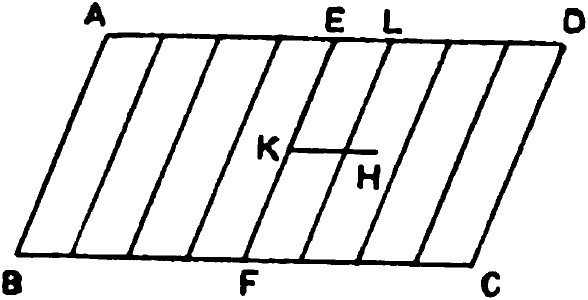
\includegraphics[scale=0.5]{Paralelogram.jpg}
			\end{figure}
			
			Pred seboj imamo torej končno mnogo enako velikih veličin, katerih težišča so po neki daljici porazdeljena ekvidistančno. Posledično se težišče celote (paralelograma $ABCD$) nahaja na daljici, ki povezuje težišči srednjih dveh manjših paralelogramov (tistih dveh, ki imata $EF$ za eno od stranic). Tukaj pa pridemo v protislovje, saj se težišče paralelograma $ABCD$, ki smo ga označili s $H$, ne nahaja znotraj omenjenih manjših paralelogramov. Sledi, da se težišče nujno nahaja na $EF$.
		\end{proof}
		Nadaljno v trditvah $13$ in $14$ težišče poljubnega trikotnika, v trditvi $15$ pa določi težišče poljubnega trapeza. 
	\section{Druga knjiga}
	
	\begin{thebibliography}{99}
		
		\bibitem{bib:Heath} T.~Heath,~\emph{A history of Greek mathematics volume $2$}, Dover Publications, New York, 1981.
		
	\end{thebibliography}
\end{document}